\documentclass[12pt]{article}

	\addtolength{\oddsidemargin}{-.5in}
	\addtolength{\evensidemargin}{-.875in}
	\addtolength{\textwidth}{1.75in}

	\addtolength{\topmargin}{-.875in}
	\addtolength{\textheight}{1.75in}

\usepackage{minted}
%\newminted[python]{python}{frame=single}
%\fvset{showspaces}
%\renewcommand\FancyVerbSpace{\textcolor{mygray}{\char32}}
\setminted[text]{
escapeinside=||, 
%breaksymbolleft=\carriagereturn,
frame=single,
%showspaces=true
framesep=2mm,
baselinestretch=1.2,
bgcolor=mygray
}
\setminted[cpp]{
escapeinside=||, 
%breaksymbolleft=\carriagereturn,
frame=single,
%showspaces=true
framesep=2mm,
baselinestretch=1.2,
bgcolor=mygray
}
\usepackage{xcolor}
\usepackage{hyperref}
\usepackage[pdftex]{graphicx}
\usepackage{multirow}
\usepackage{setspace}
\usepackage{color}
\usepackage{multicol}
\usepackage{listings}
\usepackage{color}
\usepackage[T1]{fontenc}

\hypersetup{
    bookmarks=true,         % show bookmarks bar?
    unicode=false,          % non-Latin characters in Acrobat’s bookmarks
    pdftoolbar=true,        % show Acrobat’s toolbar?
    pdfmenubar=true,        % show Acrobat’s menu?
    pdffitwindow=false,     % window fit to page when opened
    pdfstartview={FitH},    % fits the width of the page to the window
    pdftitle={My title},    % title
    pdfauthor={Author},     % author
    pdfsubject={Subject},   % subject of the document
    pdfcreator={Creator},   % creator of the document
    pdfproducer={Producer}, % producer of the document
    pdfkeywords={keyword1, key2, key3}, % list of keywords
    pdfnewwindow=true,      % links in new PDF window
    colorlinks=true,       % false: boxed links; true: colored links
    linkcolor=red,          % color of internal links (change box color with linkbordercolor)
    citecolor=green,        % color of links to bibliography
    filecolor=magenta,      % color of file links
    urlcolor=blue           % color of external links
}

\definecolor{dkgreen}{rgb}{0,0.6,0}
\definecolor{gray}{rgb}{0.5,0.5,0.5}
\definecolor{mauve}{rgb}{0.58,0,0.82}
\lstset{frame=tb,
  language=Java,
  aboveskip=3mm,
  belowskip=3mm,
  showstringspaces=false,
  columns=flexible,
  basicstyle={\small\ttfamily},
  numbers=none,
  numberstyle=\tiny\color{gray},
  keywordstyle=\color{blue},
  commentstyle=\color{dkgreen},
  stringstyle=\color{mauve},
  breaklines=true,
  breakatwhitespace=true,
  tabsize=3
}

% ME4140 - Fall 2016 - Fall 2017 - Fall 2019



\textwidth=6.5in
\topmargin=-0.5in
\textheight=9.25in
\hoffset=-0.5in
\footskip=0.2in

\pagestyle{myheadings}
\markright{{\large ME 4140 Fall 2019---The Robotic Operating System}}

\definecolor{dkgreen}{rgb}{0,0.6,0}
\definecolor{gray}{rgb}{0.5,0.5,0.5}
\definecolor{mauve}{rgb}{0.58,0,0.82}

\definecolor{mygray}{rgb}{.6, .6, .6}
\definecolor{mypurple}{rgb}{0.6,0.1961,0.8}
\definecolor{mybrown}{rgb}{0.5451,0.2706,0.0745}
\definecolor{mygreen}{rgb}{0, .39, 0}

\newcommand{\R}{\color{red}}
\newcommand{\B}{\color{blue}}
\newcommand{\BR}{\color{mybrown}}
\newcommand{\K}{\color{black}}
\newcommand{\G}{\color{mygreen}}
\newcommand{\PR}{\color{mypurple}}

\newcommand{\pkgname}{<package\_name>}
\newcommand{\wspname}{<workspace\_name>}
\newcommand{\nodname}{<node\_name>}
\newcommand{\tpcname}{<topic\_name>}
\newcommand{\lfname}{<file\_name>}

\newcommand{\home}{\textasciitilde/}

\newcommand{\rosdistro}{melodic}

\newcommand{\pthname}{/opt/ros/\rosdistro/share/turtlebot\_stage/maps/}


\begin{document}

\thispagestyle{plain}

\begin{center}
   {\bf \Large ROS - Navigation and The Turtlebot3 Simulator}\vspace{2mm} \\
   {\bf \large ME 4140 - Introduction to Robotics - Fall 2019} \\
\end{center}



What do we mean by navigation? This means different things in different places. Here, we specifically mean the naviagation stack in ROS melodic. This tutorial comes from \href{http://emanual.robotis.com/docs/en/platform/turtlebot3/simulation/#simulation} {here.}  \\

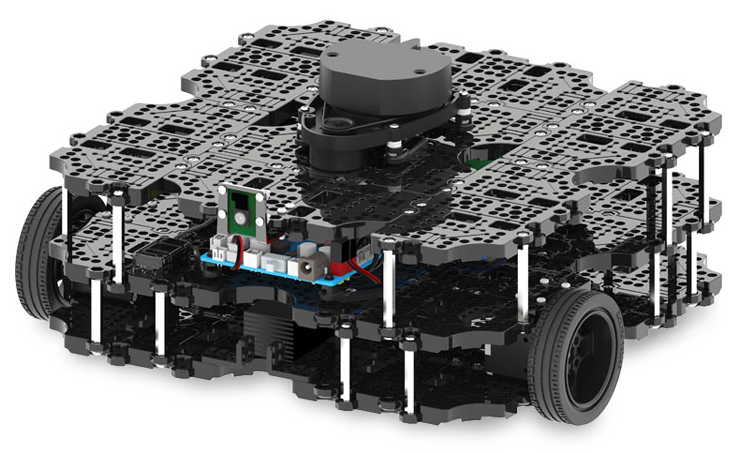
\includegraphics[scale=.20]{turtlebotPi.jpg}
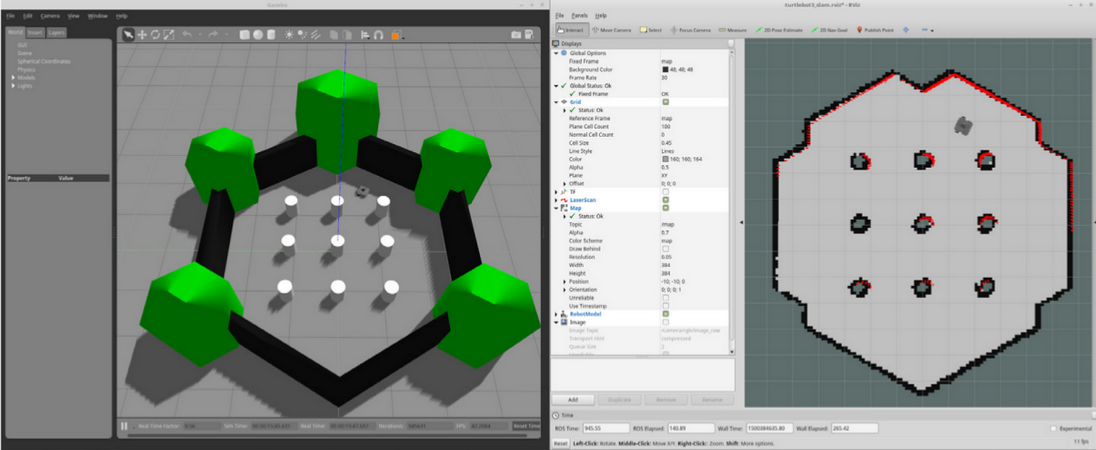
\includegraphics[scale=.25]{turtlebot3_maps.png} 

\begin{enumerate}
\item First creating a map by driving the robot in the virtual environmentwith and collecting lidar data. \\
{\bf Install the {\bf navigation} and {\bf gmapping} nodes if you have not already.}
\begin{minted}{text} 
sudo apt install ros-melodic-navigation ros-melodic-gmapping
\end{minted}
{\bf   Start the turtlebot3 simulator.}
\begin{minted}{text} 
  export TURTLEBOT3_MODEL=waffle_pi
  roslaunch turtlebot3_gazebo turtlebot3_world.launch
\end{minted}
{\bf Next, start SLAM using the gmapping node. }
\begin{minted}{text} 
 export TURTLEBOT3_MODEL=waffle_pi
 roslaunch turtlebot3_slam turtlebot3_slam.launch slam_methods:=gmapping
\end{minted}
 {\bf Drive the robot around with the keyboard to collect data/}
\begin{minted}{text} 
 export TURTLEBOT3_MODEL=waffle_pi
  roslaunch turtlebot3_teleop turtlebot3_teleop_key.launch
\end{minted}
 {\bf When you are finished save the map.}
\begin{minted}{text} 
  rosrun map_server map_saver -f ~/map
\end{minted}


%    \item Next install the physical 'turtlebot' drivers into your ROS system. This step is only necessary if you are using a real turtlebot. \href{http://wiki.ros.org/Robots/TurtleBot} {Link Here} 
%   \begin{minted}{text}  
%(sudo apt-get install ros-|\rosdistro|-turtlebot ros-|\rosdistro|-turtlebot-apps
%ros-|\rosdistro|-turtlebot-interactions ros-|\rosdistro|-turtlebot-simulator 
%ros-|\rosdistro|-kobuki-ftdi ros-|\rosdistro|-rocon-remocon 
%ros-|\rosdistro|-rocon-qt-library ros-|\rosdistro|-ar-track-alvar-msgs})
%\end{minted}xright
%    
\newpage
    \item Now that you have made a map of the space your robot can naigative autonomously using the navigation stack, a collection of packages. \\\\
{\bf   Start the turtlebot3 simulator.}
\begin{minted}{text} 
  export TURTLEBOT3_MODEL=waffle_pi
  roslaunch turtlebot3_gazebo turtlebot3_world.launch
\end{minted}
{\bf  Then turn on the navigation nodes and RVIZ. }
\begin{minted}{text} 
roslaunch turtlebot3_navigation turtlebot3_navigation.launch map_file:=$HOME/map.yaml
\end{minted}

	You should see the gazebo window open containing your robot. as well as rviz. Find and test the following features of navigation in RVIZ. \\
	
	1) Pose Estimate \\\\
	
	2) 2D Nav Goal \\\\

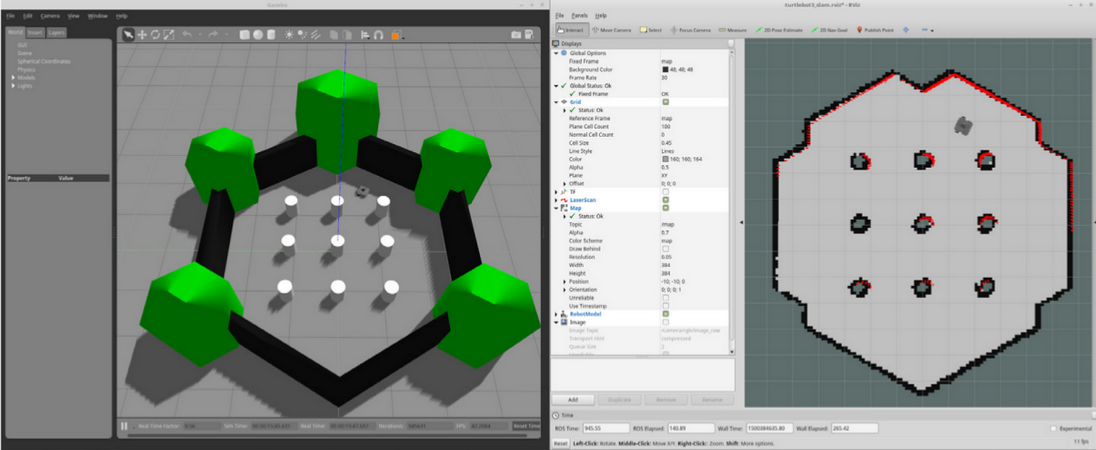
\includegraphics[scale=.40]{turtlebot3_rviz.png}
%    \begin{itemize}
%    
%        \item {\fontfamily{qcr}\selectfont  \hspace{5mm} \pthname maze.png}
%        \item {\fontfamily{qcr}\selectfont  \hspace{5mm} \pthname maze.yaml}
%        \item {\fontfamily{qcr}\selectfont  \hspace{5mm} \pthname stage/maze.world}
%    
%    \end{itemize}

%    \item First try the simulator in the demo world called {\it maze}. We will export the files as {\it environment variables}
%
%    {\fontfamily{qcr}\selectfont  \hspace{5mm} \$ export TURTLEBOT\_STAGE\_MAP\_FILE=\\"\pthname maze.yaml"}\\
% 
%    {\fontfamily{qcr}\selectfont  \hspace{5mm} \$ export TURTLEBOT\_STAGE\_WORLD\_FILE=\\"\pthname stage/maze.world"}\\
%    
%    \item Now use the launch file (available upon install) to start the simulator.\\
%    {\fontfamily{qcr}\selectfont  \hspace{5mm} \$ roslaunch turtlebot\_stage turtlebot\_in\_stage.launch}
%    
%    \item Now you can modify the world you have just simulated. To do this copy all three files and rename them something sensible. Open the {\it .png} file with any image editor, and draw on it and save. You also need to modify just a few lines in the {\it .yaml} file and the {\it .world} file. (Note: This step will be detailed in the next tutorial. Continue at your own risk or contact me for help.)
%    
%     \item Did you notice an error when you turned the node on? We can fix that.  \\\\
%    
%    	 {\fontfamily{qcr}\selectfont  \hspace{5mm} \$ sudo  gedit /opt/ros/\rosdistro/share/gmapping/nodelet\_plugins.xml}\\\\
%    	 
%    	 Copy the code below into the new file. This a bug related to moving to `kinetic'.\\
%    \lstset{language=XML}
%     \begin{lstlisting}
%
%<library path="lib/libslam_gmapping_nodelet">
%    <class name="SlamGMappingNodelet" type="SlamGMappingNodelet" base_class_type="nodelet::Nodelet">
%        <description>
%            Nodelet ROS wrapper for OpenSlams Gmapping.
%        </description>
%    </class>
%</library>
%      \end{lstlisting}
%
%\vspace{5mm}    Now run your node again.
\end{enumerate}
\end{document}

